% This file contains the content for a main section
\regularsectionformat	% Change formatting to that of "Introduction" section
%% Modify below this line %%
\chapter{Workflow Integration}

\section{Application to entire image, pixel by individual pixel}
As with all other ACES transforms, LMTs are applied across the entire image, and are not applied to any subset of the image. Similarly, as with all other ACES transforms, the outputs of the LMT depend solely on its inputs, with no contribution from neighboring regions of the image.

\section{Ubiquity}
The LMT is a key transform in the ACES system, and must be supported in any system component supporting ACES workflows that allows for image alteration. (An example of an ACES system component not allowing image alteration would be a display that interpreted its inputs as being ACESproxy values.) The ability to specify, record, transport and/or apply LMT(s) can be present in almost any component of an ACES-based workflow, including applications for converting native camera output to ACES imagery, on-set grading and dailies tools, color correctors, displays and CG tools.

\section{Optimizations}
When there are multiple LMTs making up a Look Transform, the hardware or software implementing the ACES viewing pipeline may optimize the application of the Look Transform by combining the LMTs into a single LUT; it may also combine this Look Transform LUT with the RRT and a selected ODT.

\subsection{Composite transform sampling using a 3D LUT}
Applications may also send a lattice of sample values through some set of adjacent transforms (anything from two or more adjacent LMTs in the Look Transform, to the full concatenation of Look Transform plus RRT and a selected ODT) to derive a single 3D LUT.

Artifact-free processing across the large range of ACES RGB relative exposure values requires shaper LUTs before and after the 3D LUT to minimize interpolation error.

\section{Retention}
LMTs need to be saved with every clip or project, and loaded automatically into the user's application so that the creatively established Look Transform is maintained at every step of production and post-production. Every LMT contains, as part of its description, an ACES Transform Identifier. To maintain portability of LMTs, the metadata identifying them -- their ACES Transform Identifiers -- must be included within the ACES clip container, and the order in which they are referenced in the ACES clip container `TransformList' is the order in which they should be applied.

\section{Nondestructive preview of displayed image appearance}
LMTs are one of several types of transform applied to either camera-specific files in proprietary or standard format that have been converted into ACES by an IDT, or to ACES files in OpenEXR containers. In the most general of cases, the input image data will be processed first by zero or more pre-grades, then by the grading transform, then by zero or more LMTs, then by the RRT, then by a selected ODT, and then displayed to the user. This most general case is shown in \autoref{fig:preview}.

\begin{figure}[htb]
\begin{center}
    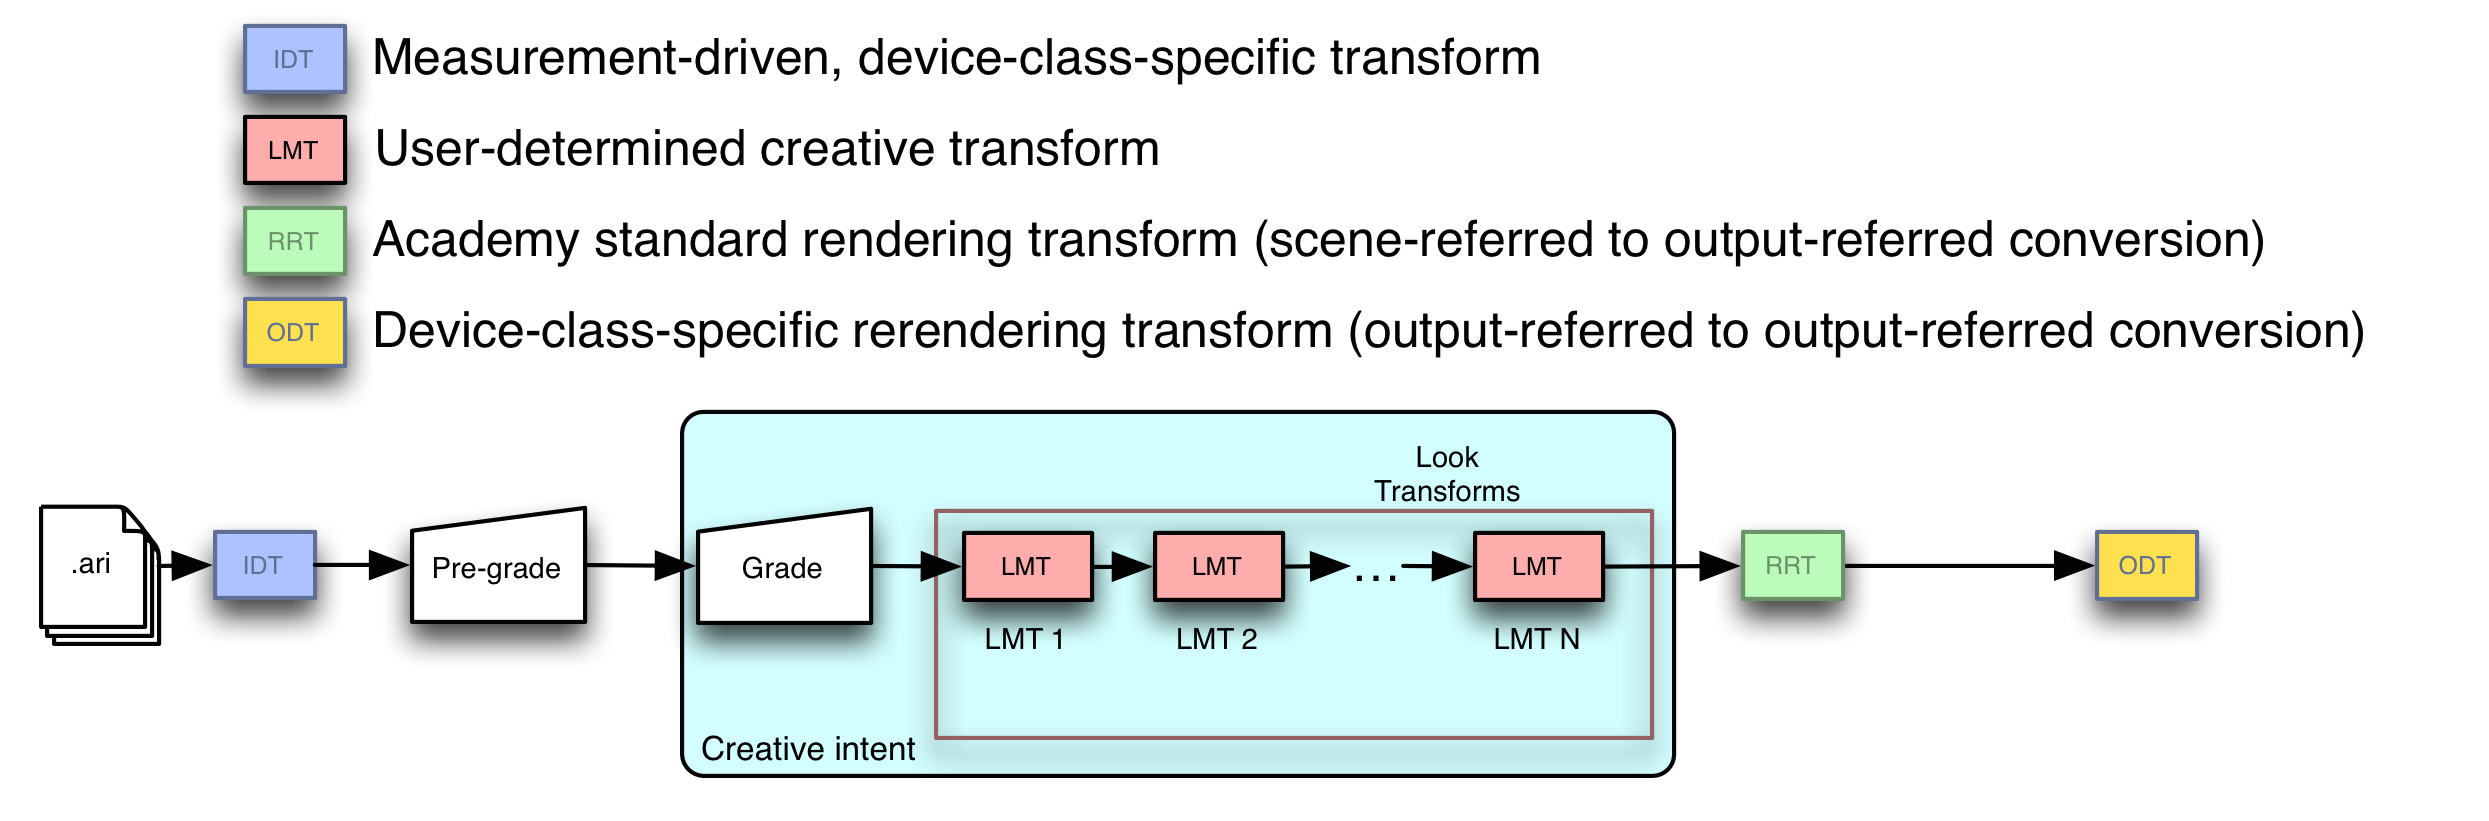
\includegraphics[width=\textwidth]{preview.png}
\caption{}
\label{fig:preview}
\end{center}
\end{figure}

The syntax and semantics of LMTs are given in the Specification section above. The syntax and semantics of pre-grading and grading operations are outside the scope of this document; indeed, they are outside the scope of the ACES project itself.

\section{Archival of ACES imagery with and without ‘baked in’ grading and/or LMT application}
Every archived ACES image has an implied associated displayed image, namely, the result of processing that archived ACES image with the RRT and the ODT that was used when creative approval was given. Because of this it is critical that the selected ODT (including all relevant versioning information) be archived alongside any archived ACES imagery, whether or not that ACES imagery is the product of `baking in' grades and/or the application of one or more LMTs making up a Look Transform.

Since many grading operations and LMTs may reduce the color volume in the original image to a smaller color volume that is then delivered to the RRT and a selected ODT, productions wishing to `future-proof' their assets should store the original ACES files, along with all pre-grading information, grading information, the ordered set of LMTs that make up the Look Transform and the ODT that was selected at the time of creative approval. (An LMT applying ASC CDL would be an example of such a color-volume-reducing transformation, as ASC CDL is applied in the ACEScc color space, a smaller color space than ACES.)